% @Author: Rishabh Pomaje
% @Email: 210020036@iitdh.ac.in

\documentclass[11pt,compress,dvipsnames,aspectratio=169, t]{beamer}

% Packages
\input{preamble/tooltips.tex}
\usepackage{tikz}
\usetikzlibrary{shapes, positioning, decorations.pathmorphing, decorations.markings, calc}

\usepackage{etoolbox}
\usepackage{amsmath, amssymb, amsfonts, mathtools, bm, mathrsfs}
\usepackage{subcaption}
\usepackage[svgnames, dvipsnames]{xcolor}
\usepackage{tcolorbox}

\newtcolorbox[auto counter]{thm}[2][]{%
  colback=red!10, 
  colframe=Maroon, 
  fonttitle=\bfseries, 
  boxrule=1pt, 
  coltitle=Seashell, 
  coltext=black, 
  left=5pt, right=5pt, top=5pt, bottom=5pt, 
  title=Theorem~\thetcbcounter: #2,#1
}
\newtcolorbox[auto counter]{prop}[2][]{%
  colback=green!10, 
  colframe=DarkGreen,
  fonttitle=\bfseries, 
  boxrule=1pt, 
  coltitle=Seashell, 
  coltext=black, 
  left=5pt, right=5pt, top=5pt, bottom=5pt, 
  title=Proposition~\thetcbcounter: #2,#1
}
\newtcolorbox[auto counter]{clm}[2][]{%
  colback=teal!10, 
  colframe=teal!10, 
  fonttitle=\bfseries, 
  boxrule=1pt, 
  sharp corners, 
  coltitle=teal, 
  coltext=black, 
  left=5pt, right=5pt, top=5pt, bottom=5pt, 
  title=Claim,
}

\newtcolorbox[auto counter]{nt}[2][]{%
  colback=black!10, 
  colframe=black!75, 
  fonttitle=\bfseries, 
  boxrule=1pt, 
  coltitle=Seashell, 
  coltext=black, 
  left=5pt, right=5pt, top=5pt, bottom=5pt, 
  title=Note
}

\newtcolorbox{MyButton}[1][]{%
  enhanced,
  box align=base,
  colback=gray!10,
  colframe=black,
  colupper=black,
  fontupper=\fontsize{6pt}{10pt}\selectfont\bfseries,
  boxrule=2pt,
  % arc=4pt,
  sharp corners,
  top=0.5pt,
  bottom=0.5pt,
  left=4pt,     % tighter horizontal padding
  right=4pt,    % tighter horizontal padding
  % drop shadow southeast,
  % interior style={top color=blue!25, bottom color=Azure},
  valign=center,
  halign=center,
  nobeforeafter,
  boxsep=0pt,   % removes inner spacing between content and box border
  hbox,
  underlay vignette,
  #1
}

\newcommand{\Button}[1]{%
  \begin{MyButton}
    \strut#1%
  \end{MyButton}%
}

\usepackage{hyperref}
\hypersetup{
    % pdfbookmarks=true,
    colorlinks=true, 
    linkcolor=NavyBlue, 
    urlcolor=Mahogany, 
    citecolor=green, 
    filecolor=magenta 
}



% Theme settings
\usetheme{boadilla}
\useinnertheme{circles}
\usefonttheme{professionalfonts}
\setbeamercovered{transparent} 
\usepackage{libertinus}

\setbeamercolor{title}{fg=MidnightBlue, bg=AliceBlue}
\setbeamercolor{subtitle}{fg=Black}
\setbeamercolor{alerted text}{fg=Red}
\setbeamercolor{frametitle}{fg=MidnightBlue, bg=AliceBlue}
\setbeamercolor{normal text}{fg=Black, bg=White}
\setbeamercolor{item}{fg=Navy}
\setbeamercolor{block title}{fg=AliceBlue, bg=MidnightBlue}
\setbeamercolor{block body}{fg=Black, bg=AliceBlue}
\setbeamercolor{title in head/foot}{fg=Black, bg=AliceBlue}
\setbeamercolor{date in head/foot}{fg=Black, bg=AliceBlue}
\setbeamercolor{institute in head/foot}{fg=Black, bg=AliceBlue}
\setbeamercolor{author in head/foot}{fg=Black, bg=AliceBlue}

\setbeamertemplate{navigation symbols}{}
\renewcommand\qedsymbol{$\diamondsuit$}

% Add logo to every page
\addtobeamertemplate{frametitle}{}{%
  \begin{textblock*}{3cm}(15.2cm,0.1cm)
    \includegraphics[width=0.5cm]{property/tree_logo.pdf} % Make sure logo file is in the same folder
  \end{textblock*}
}

\usepackage[absolute,overlay]{textpos}

% Title and Author Information
\title[Course/Conference/Seminar]{\textbf{Main Title Goes Here}}
\author[]{Rishabh Pomaje\inst{1}\\ \small Supervisor, Co-Author: Name01\inst{1}, Name02\inst{2}
}
\institute[Stanford University]{
  \inst{1}Dept. Electrical Engineering,
  Stanford University, CA.\\
  \inst{2}Department of Computer Science, University of \LaTeX, \TeX.
}

\date[\today]{\today}
\begin{document}

\begin{frame}
  \titlepage
\end{frame}

\section{Introduction}
\begin{frame}{Motivation}
  \begin{itemize}
    \item Wireless networks demand efficient learning strategies.
    \item Deep learning enables adaptive modulation, resource allocation.
    \item Goal: Reduce latency and improve robustness.
  \end{itemize}
\end{frame}

\section{Results}
\begin{frame}{Simulation Results}
  \begin{columns}
    \column{0.5\textwidth}
      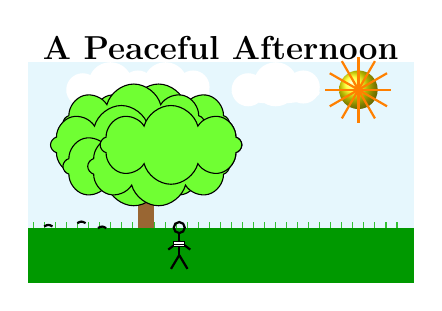
\begin{tikzpicture}[scale=0.35]
        % Sky background
        \fill[cyan!10] (0,0) rectangle (14,8);

        % Sun
        \shade[ball color=yellow] (12,7) circle (0.7);
        \foreach \i in {0,30,...,330}
          \draw[orange, thick] (12,7) -- ++(\i:1.2);

        % Clouds
        \foreach \x in {3, 5, 9} {
          \begin{scope}[shift={(\x,7)}]
            \fill[white] 
              (-1,0) circle (0.6) 
              (0,0.2) circle (0.8) 
              (1,0.1) circle (0.6) 
              (0,-0.1) ellipse (1.6 and 0.4);
          \end{scope}
        }

        % Grass
        \fill[green!60!black] (0,0) rectangle (14,2);
        \foreach \x in {0.2, 0.6,...,13.8} {
          \draw[green!70!black!80!white] (\x,2) -- ++(0,0.2);
        }

        % Tree trunk
        \fill[brown!80!black] (4,2) rectangle (4.6,5);

        % Tree leaves (top)
        \foreach \i in {0,1,...,6} {
          \path[shift={(4.3,5)}] 
            ++(60*\i:0.9) 
            node[cloud, cloud puffs=8, draw, minimum width=1.8cm, minimum height=1cm, fill=green!60!lime!80!white] {};
        }

        % Stick figure under the tree
        \begin{scope}[shift={(5.5,2)}]
          \draw[thick] (0,0) circle (0.2);        % Head
          \draw[thick] (0,-0.2) -- (0,-1);        % Body
          \draw[thick] (0,-0.5) -- (-0.4,-0.8);   % Left arm
          \draw[thick] (0,-0.5) -- (0.4,-0.8);    % Right arm
          \draw[thick] (0,-1) -- (-0.3,-1.5);     % Left leg
          \draw[thick] (0,-1) -- (0.3,-1.5);      % Right leg
          % Book
          \draw[fill=white] (-0.2,-0.7) rectangle (0.2,-0.5);
          \draw (-0.2,-0.6) -- (0.2,-0.6);
        \end{scope}

        % Bird in sky
        \foreach \x/\y in {2/6.8, 6/7.2, 8.5/6.6} {
          \draw[scale=0.3, thick] (\x,\y) .. controls +(30:0.5) and +(150:0.5) .. ++(1,0);
        }

        % Title
        \node[font=\large\bfseries] at (7,8.5) {A Peaceful Afternoon};

      \end{tikzpicture}
    \column{0.5\textwidth}
      \begin{itemize}
        \item Proposed method outperforms baseline
        \item Faster convergence and better reliability
      \end{itemize}
  \end{columns}
\end{frame}

\section{Conclusion}
\begin{frame}{Conclusion and Future Work}
  \begin{itemize}
    \item Presented a DNN-based framework for real-time decision making
    \item Next steps: real hardware testbed validation
  \end{itemize}
\end{frame}

\begin{frame}{Any Questions?} 
  \centering

  \vspace{1.5cm}

  {\Huge \textbf{\textcolor{Mahogany}{Thank You!}}} 

  \vspace{2cm}

  {\small
      \textbf{Rishabh Pomaje} \\
      \textcolor{NavyBlue}{Email: \href{rishabhp@stanford.edu}{rishabhp@stanford.edu}} \\
      % \textcolor{NavyBlue}{Phone: +91-9834924475}
  }
\end{frame}

\end{document}
